\subsection{Цепь Маркова}

Разобьем время на слоты длительности $\tau = \gcd(\Tres,\Tin)$ таким образом, чтобы начало каждого зарезервированного интервала совпадало с началом некоторого слота. Затем выразим $\Tres$ и $\Tin$ в слотах:

\begin{center}
$\tres = \frac{\Tres}{\tau}, \tin = \frac{\Tin}{\tau}, ~~\tres, \tin \in \mathbb{N}.$
\end{center}

Будем моделировать процесс передачи с помощью цепи Маркова с дискретным временем, для этого будем наблюдать процесс в начале каждого зарезервированного интервала. 

\begin{figure}[h]
\centering{
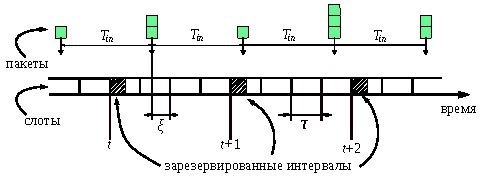
\includegraphics[width=\linewidth]{MarkChain.pdf}
\caption{\label{fig:Mark}Дискретное время цепи Маркова}}
\end{figure}

В моменты наблюдения процесс описывается тремя целыми числами $(h,m,r)$. $h$ -- это время, которое самый старший пакет провел в очереди, выраженное  в слотах и округленное вниз. Если очередь пуста, то формально полагается, что $h < 0$, причем $h$ равно времени до прибытия следующей пачки, взятому со знаком минус, выраженному в слотах и округленному вниз. $m$ -- это число оставшихся в головной пачке пакетов (либо число пакетов в еще не пришедшей пачке, если очередь пуста). $r$ представляет собой оставшееся число попыток передач для головного пакета.

%If $\tres \le \tin$ the minimal value of $h$ equals $\tres - \tin$. It is reached at instance $t+1$ when a) the batch of a single packet arrives into the empty queue at instance $t$ right before the beginning of a reserved interval and b) is successfully transmitted in this interval.  Otherwise, if $\tres > \tin$, then the minimal value equals $0$. 

Из определения $h$ следует, что эта величина всегда больше чем $-\tin$: следующая пачка пакетов поступает в очередь не позже чем через $(\tin - 1)$ слотов. $h$ определяет время жизни самого старшего пакета в очереди (самой старшей пачки пакетов). Чтобы определить верхнюю границу для $h$, введем величину $\xi$, равную длительности промежутка времени между моментом, когда пачка поступает в очередь, и началом следующего слота ($\xi$ всегда одинакова для всех пачек по определению слота). Виртуально сдвинем все моменты поступления пакетов на время $\xi$ вперед к началам ближайших слотов, уменьшив при этом величину $\DQoS$ на $\xi$. Это не повлияет на процесс передачи, так как такой сдвиг приводит лишь к тому, что каждый поступающий пакет простаивает в течение времени $\xi$ после поступления в очередь. Пусть очередь непуста, тогда время $t$, которое пакеты головной пачки провели в очереди, есть $h\tau$. Из-за ограничения на время жизни пакета всегда выполняется неравенство $h(t)\tau \leq \DQoS$, откуда получаем $h \leq d = \lfloor \frac{\DQoS}{\tau} \rfloor$.   

Пусть процесс находится в состоянии $(h(t),m(t),r(t))$ в момент $t$. Найдем все возможные переходы между состояниями цепи Маркова. 

\noindent\paragraph{\bm{$h(t) < 0.$}} В этом случае очередь пуста и следующая пачка поступит в очередь через $|h(t)|$ слотов. $m(t)$ представляет собой размер этой <<будущей>> пачки, а $r(t) = \nretries$, поскольку головной пакет из <<будущей>> пачки еще ни разу не был передан.
%This case corresponds to the empty queue. In this case $r(t) = \nretries$ and $m(t)$ is the size of future batch. 
При этом процесс с вероятностью 1 перейдет в состояние $(h(t)+\tres,m(t),r(t))$.
%If $\tres < |h(t)|$, before the beginning of the next reserved interval the queue will be still empty and the value of $h(t+1)$ is equal to $h(t) + \tres$. Otherwise, if $\tres \geq |h(t)|$, then there will be a pack in the queue before the beginning of the next reserved interval and the amount of time which this pack spent in queue is equal to $h(t) + t_{res}$. As for other parameters, they stay unaltered during this transition. In this way, if $h(t) < 0$, the system always has a transition to state  
\noindent\paragraph{\bm{$0 \leq h \leq d - \tres.$}} В этом случае очередь непуста, и пакеты головной пачки не устареют к следующему зарезервированному интервалу. Возможные переходы зависят от значений $m(t)$ и $r(t)$.
\begin{itemize}
\item $\bm{m(t) = 1}$ и $\bm{r(t) > 1.}$ Если попытка передачи была успешной (с вероятностью $1-\perm$), то головная пачка покинет очередь, поскольку состоит из единственного пакета. Размер следующей пачки равен $j$ с вероятностью $\pin_j$. Так как следующая пачка поступает в очередь через $\tin$ слотов, процесс перейдет в состояние $(h(t) - \tin + \tres, j, \nretries)$ с вероятностью $(1-\perm)\pin_j$. В противном случае при неуспешной передаче процесс перейдет в состояние $(h(t) + \tres, m(t), r(t) - 1)$ с вероятностью $\perm$.
%means that there is one packet left in the head pack and it still has some retries to transmit. Possible transitions from this state are to $(h(t) - \tin + t_{res}, m_{i}, \mathcal{R})$ with probability $p(m_{i})*(1-q_{m})$ if there was a successful transmission of this single packet and the queue got another pack with random amount of packets $m_{i}$, and to $(h(t)+ t_{res}, m(t), r(t) - 1)$ with probability $q_{m}$ if the transmission was unsuccessful and the packet was left in the queue.
\item $\bm{m(t) = 1}$ и $\bm{r(t) = 1}$. В этом случае последний пакет головной пачки в любом случае покинет очередь по причине достижения предельного количества попыток передач. Таким образом, процесс перейдет в состояние $(h(t) - \tin + \tres, j, \nretries)$ с вероятностью $\pin_j$.
\item $\bm{m(t) > 1}$ и $\bm{r(t) > 1}$. Если попытка передачи была успешной (с вероятностью $1-\perm$), процесс перейдет в состояние $(h(t)+\tres, m(t)-1, \nretries)$. В противном случае процесс перейдет в состояние $(h(t)+\tres, m(t), r(t) - 1)$ (с вероятностью $\perm$). 
% means that the head packet is not the last in the pack and it still has some retries to transmit. Possible transitions from this state are to $(h(t) + t_{res},m(t)-1,\nretries)$ with probability $1 - q_{m}$ if the packet was successfully transmitted, and to $(h(t)+t_{res},m(t),r(t)-1)$ with probability $q_{m}$ otherwise.
\item $\bm{m(t) > 1}$ и $\bm{r(t) = 1}$. В данном случае головной пакет совершает последнюю попытку передачи, после которой он точно покинет очередь. Поэтому процесс перейдет в состояние $(h(t)+\tres,m(t)-1,\nretries)$ с вероятностью 1.
\end{itemize}

\noindent\paragraph{$\bm{d - \tres < h \leq d.}$} В этом случае головная пачка в любом случае покинет очередь к следующему зарезервированному интервалу по причине превышения ограничения на время жизни. 
%Кроме того, $\kh = \lceil \frac{h(t) - d + \tres}{\tin} \rceil - 1$ пачек следующих за головной пачкой также устареют к следующему зарезевированному интервалу. 
Процесс перейдет в состояние $(h(t) - \tin + \tres, j, \nretries)$ с вероятностью $\pin_j$.  

Теперь можно построить матрицу переходных вероятностей и найти стационарное распределение вероятностей $\bm{\pi_{(h,m,r)}}$ для состояний цепи Маркова. 
%Заметим, что переходы никак не зависят от использования механизма случайного доступа, так как он применяется только к пакетам, которые однозначно устареют к началу следующего зарезервированного интервала. 
%\begin{table}[H]
%\centering
%\caption{Possible transitions from state $(h, m, R
%)$}
%\label{}
%\begin{tabular}{|c|c|c|c|}
%\hline
%Final state 							& 	Probability 			& 	\multicolumn{2}{c|}{Condition}        		\\ \hline
%$(h + t_{res}, m, r)$                                            	&	1  				& 	\multicolumn{2}{c|}{$h < 0$}                 	\\ \hline
%$(h - \tin + t_{res},m_{i},\mathcal{R})$             	&	$p(m_{i})(1-q_{m})$	& 	\multirow{6}{*}{$0 \leq h \leq d - t_{res}$}	&	\multirow{2}{*}{$m =1, r > 1$}	\\ \cline{1-2}
%$(h + t_{res},m,r-1)$            				& 	$q_{m}$             		&                    						&						\\ \cline{1-2} \cline{4-4} 
%$(h - \tin + t_{res},m_{i},\mathcal{R})$             	&  	$p(m_{i})$            		&                  							&	$m = 1, r = 1$              		\\ \cline{1-2} \cline{4-4} 
%$(h+t_{res},m-1,\mathcal{R})$                          	& 	$1 - q_{m}$             	&                   						& 	\multirow{2}{*}{$m>1, r > 1$} 	\\ \cline{1-2}
%$(h+t_{res},m,r-1)$                                            	& 	$q_{m}$         		&                   						&						\\ \cline{1-2} \cline{4-4} 
%$(h+t_{res},m-1,\mathcal{R})$                                  & 	1             			&                  							&  	$m>1, r = 1$                 		\\ \hline
%$(h - (k+1)\tin + t_{res},m_{i},\mathcal{R})$    	& 	$p(m_{i})$ 			&	\multicolumn{2}{c|}{$d - t_{res} < h \leq d$}	\\ \hline
%\end{tabular}
%\end{table}